\chapter{Planteamiento del algoritmo en software}
\section{Recopilacion de los datos}
Para la recopilacion de los datos se utilizara la libreria wfdb que se encarga de proporcionar
funciones para leer y escribir archivos de diferentes formatos que contienen señales biomédicas,
como archivos de registro de señales (por ejemplo, formato .dat), archivos de anotaciones
 (por ejemplo, formato .atr) y archivos de cabecera (por ejemplo, formato .hea).

 Los pacientes vienen identificados por un id (por ejemplo, 101) y hay 3 ficheros por paciente, 
 con extensiones .dat, .atr y .hea

Se descarga la base de datos con la funcion de la libreria de wfdb, dldatabase que recoge 
la señal del paciente y las anotaciones de los cardiologos sobre cada pico QRS.


\lstset{language=python, breaklines=true, basicstyle=\footnotesize}
\begin{lstlisting}[frame=single]
#download the database if not available
if os.path.isdir("mitdb"):
	print('You already have the data.')
else:
	wfdb.dl_database('mitdb', 'mitdb')
\end{lstlisting}

Los pacientes de la base de datos se han hecho una prueba de 30 mins lo que en la señal 
equivale a 650000 samples.

\lstset{language=python, breaklines=true, basicstyle=\footnotesize}
\begin{lstlisting}[frame=single]
sampfrom = 0
sampto = 650000
record = wfdb.rdsamp('mitdb/102', sampfrom=sampfrom, sampto=sampto)
annotation = wfdb.rdann('mitdb/102', 'atr', sampfrom=sampfrom, sampto=sampto)
\end{lstlisting}

Por ultimo, para visualizar esta señal con las anotaciones de los cardiologos y poder comparar 
con las anotaciones que realiza el algoritmo se usara la libreria matplotlib.pyplot.

Con esto se mostrara la señal original con las anotaciones y la señal filtrada con las anotaciones
del algoritmo como en \Cref{fig:102filtradoysinfiltrar}

\lstset{language=python, breaklines=true, basicstyle=\footnotesize}
\begin{lstlisting}[frame=single]
#plot the signal
#add markers to the original signal
ax[0].plot(original_signal)
ax[1].plot(filtered_signal)
ax[0].set_xlabel('Samples')
ax[0].set_ylabel('Lead I')
ax[1].set_xlabel('Samples')
ax[1].set_ylabel('Lead I')


#Making the upper signal
for pos, sym in zip(annotation.sample, annotation.symbol):
    pos -= sampfrom
    ax[0].plot(pos, original_signal[pos], 'go', markersize=4, markerfacecolor='white')
    if(sym == "A" or sym == "V" or sym == "a"):
        ax[0].text(pos+10, original_signal[pos], sym, color='red')
    else:
        ax[0].text(pos+10, original_signal[pos], sym, color='orange')
\end{lstlisting}

\section{Filtrado de la señal original}
Este filtrado es llevado a cabo por el filtrado IIR.

El filtrado IIR, que significa "Infinite Impulse Response" (respuesta infinita al impulso),
es un tipo de filtro utilizado en el procesamiento de señales digitales y analógicas.

La formula que se utilizara para el filtrado es

\[ Y[i] = \sum_{k=0}^{N_x -1} b_k \cdot x[i-k] \]

Con lo que b son los coeficientes y x la señal a filtrar

Los coeficientes se trata de un buffer de 99 valores en punto flotante simetricos que se iteran de forma 
circular, con lo que despues de ejecutar el ultimo valor vuelve de nuevo al primero.  

Para el filtrado se usa la funcion lfilter de la libreria scipy.signal

\lstset{language=python, breaklines=true, basicstyle=\footnotesize}
\begin{lstlisting}[frame=single]
    filtered_signal = lfilter(filter_taps_99_6_28, 1.0, original_signal)
\end{lstlisting}
TODO a y formula completa ademas de una mejor explicacion

\section{Detección de picos QRS}

El algoritmo de deteccion de picos esta representada en esta funcion que 
recibe la señal filtrada e intenta detectar los picos QRS.

Este algoritmo esta basado en el que se usa en el documento  https://www.mdpi.com/2079-9292/10/19/2324 
donde en el 4.1.2 muestran una maquina de estados del proceso que realizan.

\begin{figure}[h!]
    \centering
    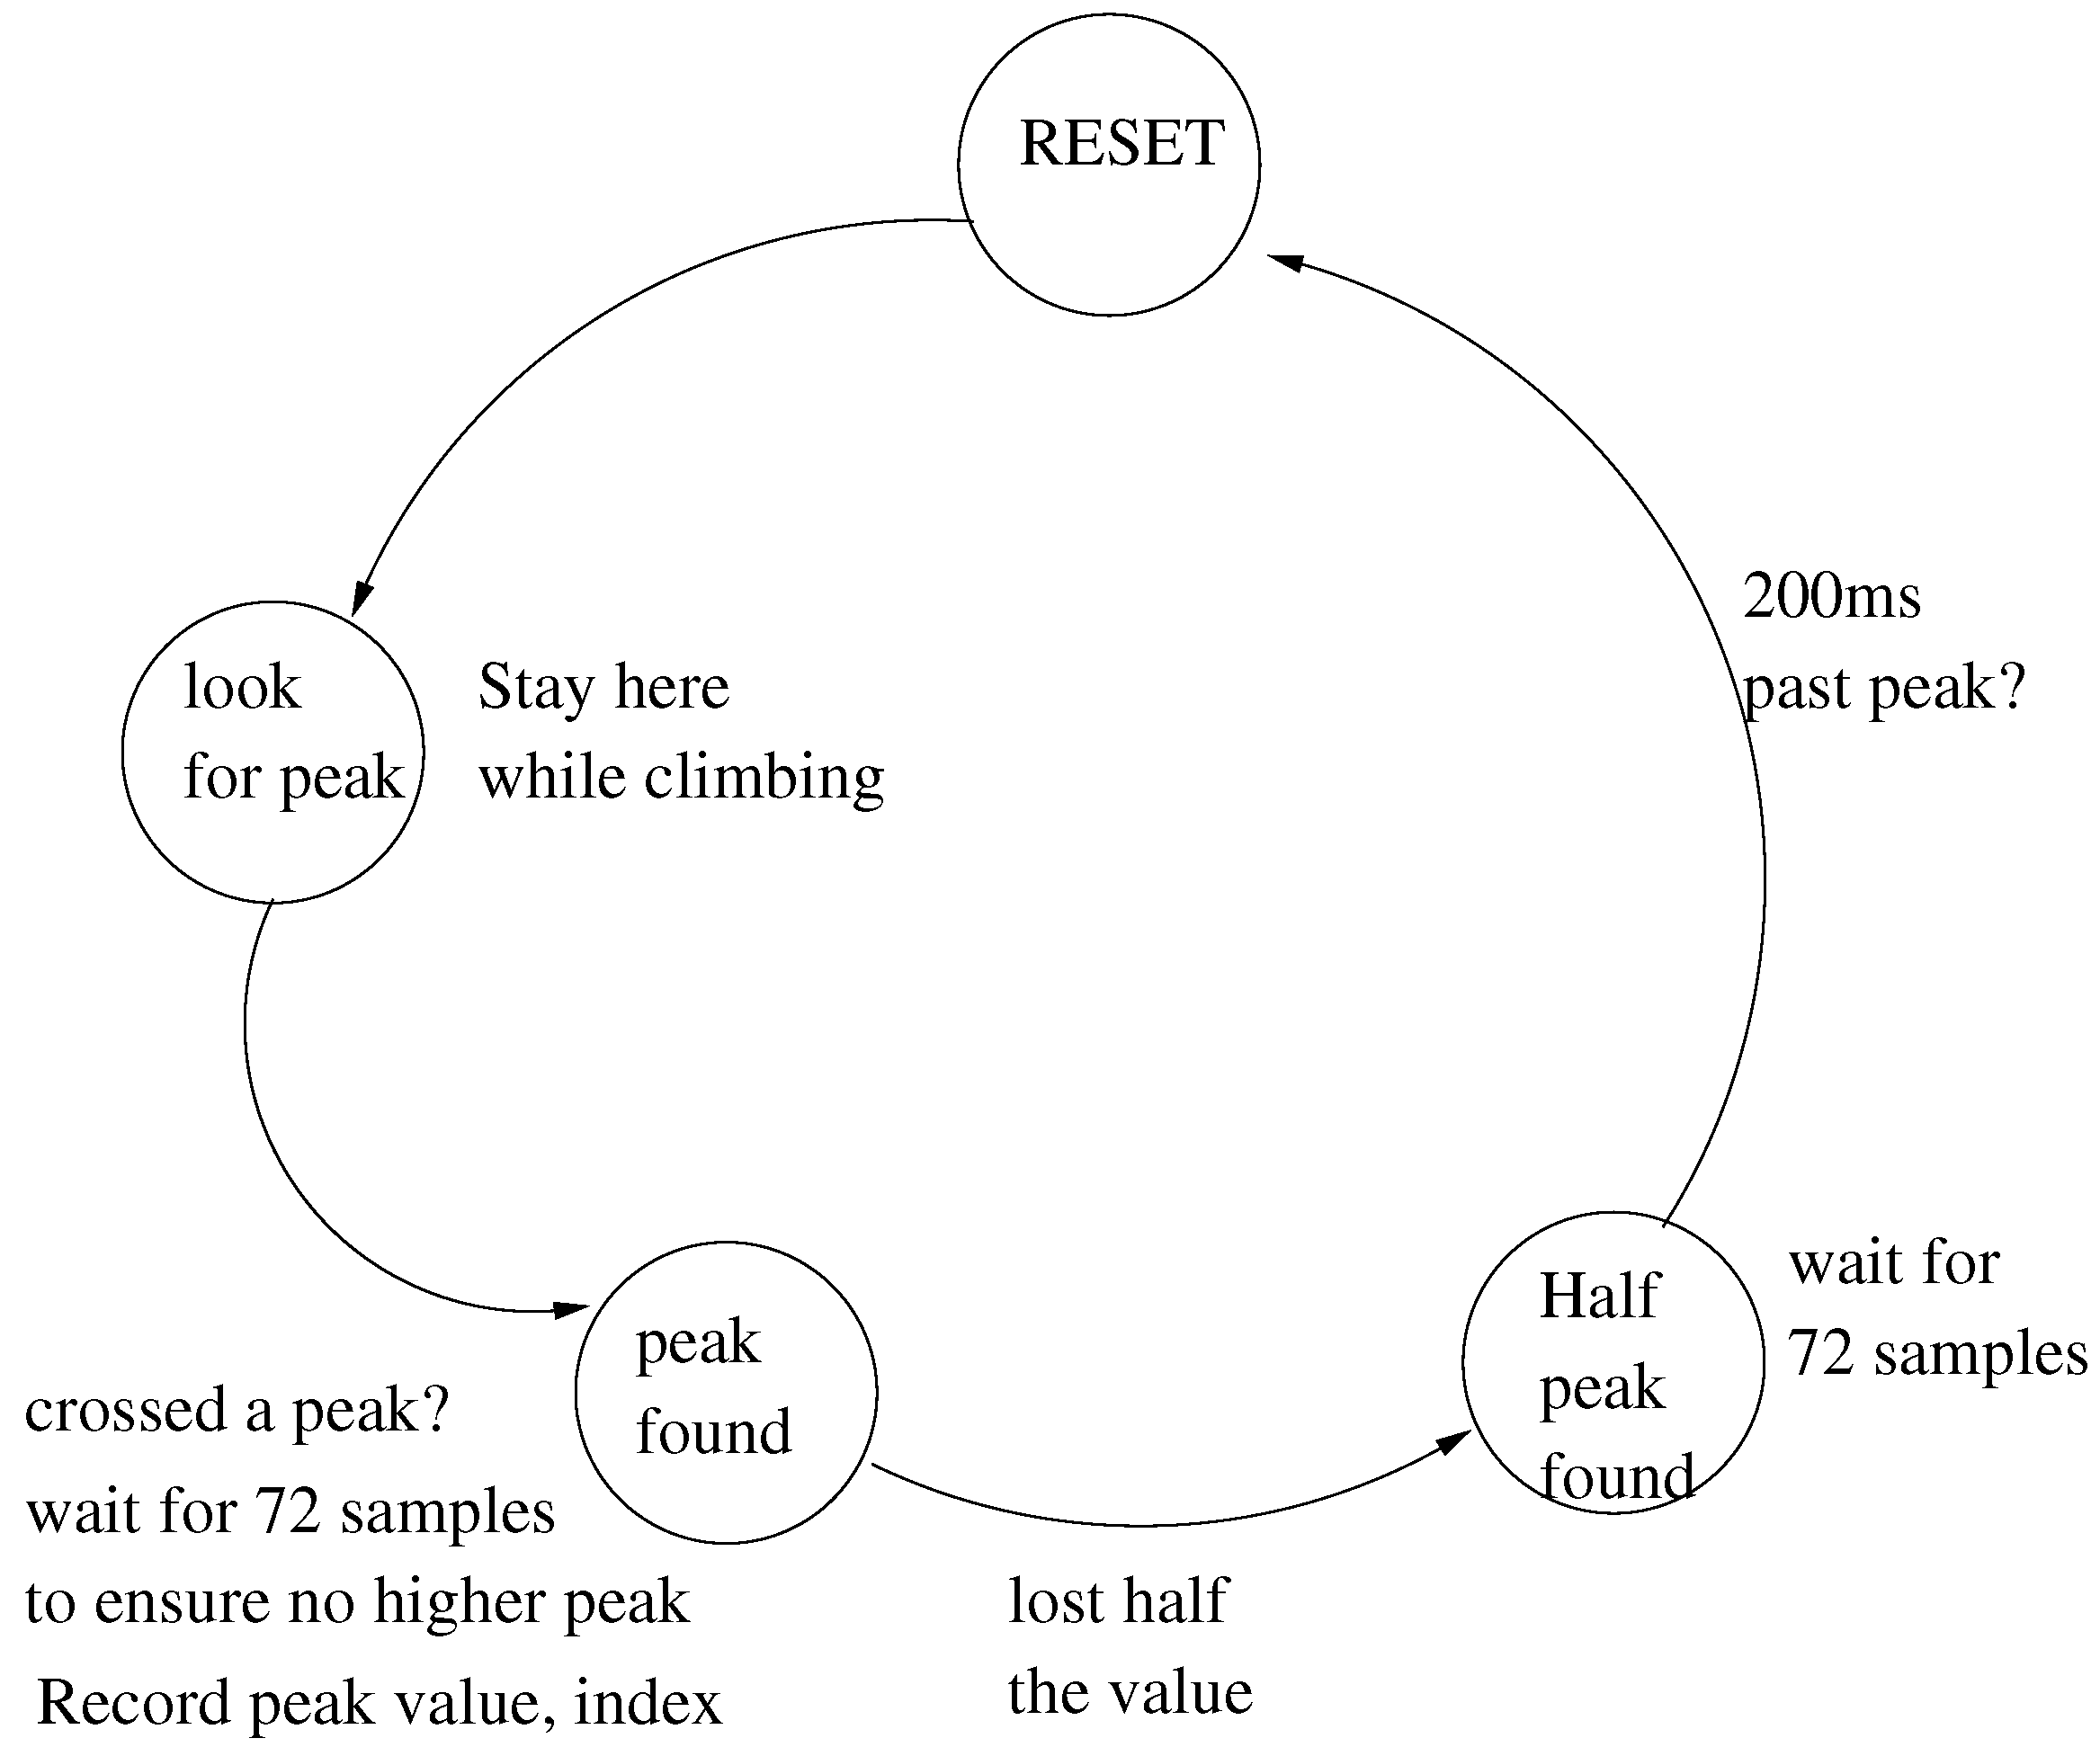
\includegraphics[width=0.6\textwidth]{./Images/img_algoritmo/fsm_mdpi.png}
    \caption{Maquina de estados de algoritmo de deteccion de picos de estudio de caracterizacion de señales usando polinomios de Hermite}
    \label{fig:fsm_mpdi}
\end{figure}

Si bien nuestro algoritmo es distinto a ese, se replica el esperar a 72 muestras
para asegurar de que no se encuentra un pico superior y asi considerarlo como un pico QRS.

Es por ello que definimos la variable \lstinline|samples_around_peak| como 72 para comparar dicha condición.

Para hallar el pico mas alto se necestia definir un pico en last\_peak y si se encuentra otro pico se produce

\lstset{language=python, breaklines=true, basicstyle=\footnotesize}
\begin{lstlisting}[frame=single]
last-peak = max(last-peak,signal[i])
\end{lstlisting}

Sin embargo hay un problema y es que cuando se detecte un pico QRS, es decir cuando se haya detectado el pico 
mas alto despues de haber pasado 72 samples se restauran los valores para empezar a detectar nuevos picos y al
haber ruido el algoritmo podria detectar falsos picos QRS asi que por ello se implementa un cutoff.

El cutoff es representado como una funcion descendente que parte de cada pico localizado y mientras no se haya
encontrado ningun pico, el valor de dicha funcion va decreciendo. La principal funcion del cutoff es evitar que
el algoritmo detecte picos con el ruido y por ello se ha ajustado para que no ocurra el problema anterior y 
ser capaz de detectar todos los picos QRS.

La funcion del cutoff es la siguiente.
\lstset{language=python, breaklines=true, basicstyle=\footnotesize}
\begin{lstlisting}[frame=single]
def calcular_cutoff(cutoff):
    cutoff = cutoff - cutoff/(256 - 64)
    return cutoff
\end{lstlisting}

Esta funcion es llamada cuando no se ha encontrado un nuevo pico y decrementa su valor, cuando se localiza un
nuevo pico, el cutoff pasa a tener el valor del pico localizado.

Se han dado los valores (256 - 64) a la formula para que fuese mas facil la divison en hardware pero como al final 
se acabo haciendo en un modulo de division en punto flotante cualquier valor es valido para la division aunque debido 
al buen desempeño del valor en el programa se decidio dejar asi.

\lstset{language=python, breaklines=true, basicstyle=\footnotesize}
\begin{lstlisting}[frame=single]
    def extract_peak_indices(signal, total_samples):
        samples_around_peak = total_samples // 2
        last_peak = None
        last_index = None
        peak_indices = []
        cutoff = 0
        for i in range(samples_around_peak-1, len(signal)):
            if last_peak == None:
                last_peak = signal[i]
                last_index = i
                cutoff = calcular_cutoff(cutoff)
            else:
                if signal[i] > last_peak and signal[i] > cutoff:
                    last_peak = signal[i]
                    last_index = i
                    cutoff= signal[i]
                else:
                    if (i - last_index) >= samples_around_peak and last_peak > cutoff:
                        peak_indices.append(last_index)
                        cutoff = calcular_cutoff(cutoff)
                        last_peak = None
                        last_index = None         
                    else:
                        cutoff = calcular_cutoff(cutoff)
            cutoff_plot.append(cutoff)
        ax[1].plot(range(samples_around_peak-1, len(signal)),cutoff_plot)
        return peak_indices
\end{lstlisting}

La salida de dicha funcion es un buffer de samples que sirven como indices para indicar donde se han encontrado
los picos QRS y asi poder pasar al modulo de deteccion de arritmias.

\section{Detección de arritmias}

El algoritmo de deteccion de arritmias se encarga de ver si se ha producido una arritmia segun la
distancia entre los picos.

En la deteccion de arritmias es de vital importancia establecer un límite en la distancia entre los picos
para poder considerar que ha habido una arritmia o no, esta tarea solo se pudo hacer probando con diferentes
rangos y viendo el indice de aciertos producidos en las pruebas a cada paciente de las que se hablara más adelante. 

El algoritmo va almacenando distancias entre los picos QRS (es por ello que en la primera iteración no se almacena nada)
y se declaran varias variables.

\begin{itemize}
    \item last\_distance: se utiliza para almacenar la ultima distancia recogida y asi poder compararla con la distancia 
    actual en calculos posteriores
    \item counter\_buffer: utilizado para tener el valor de la posicion del buffer donde se escribe.
    \item counter\_arrythmia: utilizado para indicar si la distancia anterior fue una arritmia.
    \item TNRange: Se utiliza para indicar si hay una distancia mas grande de lo normal entre 2 picos QRS producido
    por una arritmia. Es importante tener esta distancia en cuenta ya que si el ritmo del paciente vuelve a la
    normalidad se compararia la distancia entre el ritmo normal del paciente con el ritmo extendido por la arritmia,
    ya que de no tenerlo en cuenta el algoritmo lo clasificaria como arritmia como se puede ver en la \cref{fig:senial_explicacion_TNRANGE}, por ello se compara con un valor anterior
    que sea el ritmo normal del paciente.
\end{itemize}

\begin{figure}[h!]
    \centering
    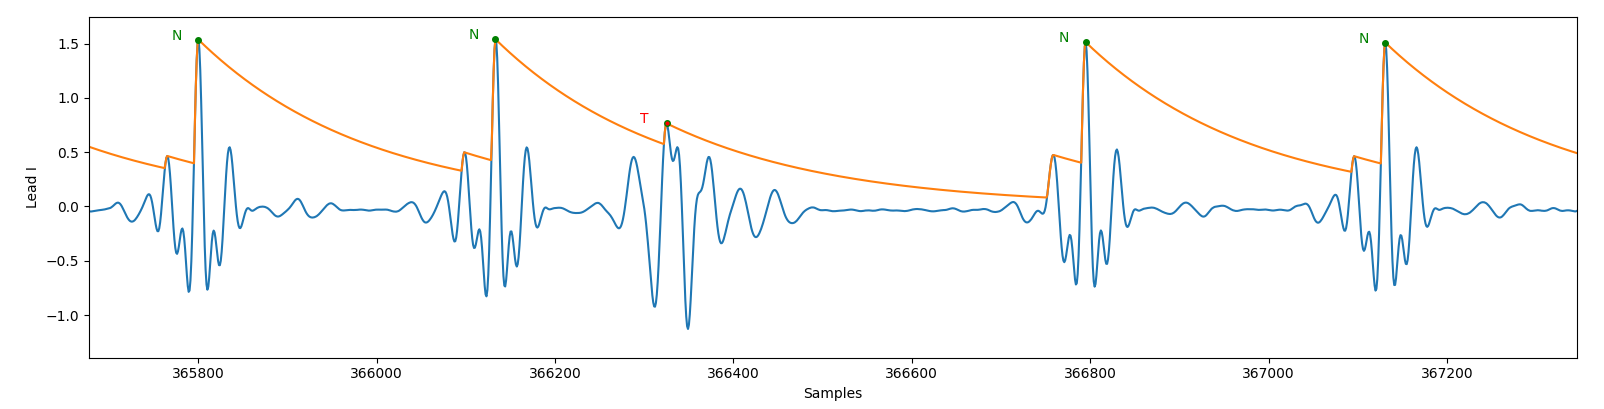
\includegraphics[width=0.9\textwidth]{./Images/img_algoritmo/senial_explicacion_TNRANGE.png}
    \caption{Cuando se detecta una arritmia, a veces, la siguiente distancia es considerablemente mas grande de lo normal. Para no detectar falsos positivos, se omite esa distancia}
    \label{fig:senial_explicacion_TNRANGE}
\end{figure}

Por ello si se ha detectado una arritmia, la siguiente distancia se compara con
la tercera ultima distancia escrita en el buffer que posiblemente sea una distancia causada por un ritmo normal. 
Si no se da el caso, se compara con last\_distance.

la funcion que compara las distancias devuelve un char que va a ser el que se vaya a plotear en la grafica, 
si el char es "N" significa que se ha detectado un ritmo normal y por tanto solo se plotea. Sin embargo si el 
resultado es "T" significa que la distancia es mas corta de lo normal, se detecta la arritmia y se ponen
counter\_arritmia a 1 para saber que la distancia es mas corta y TNRange a true para que el algoritmo sepa 
que la distancia que venga despues puede ser una ampliada. 

\lstset{language=python, breaklines=true, basicstyle=\footnotesize}
\begin{lstlisting}[frame=single]
    #init the first distance, the first beat doesn't count
    posant = peaks[0]
    last_distance = peaks[1] - peaks[0]

    pos_buffer = [last_distance]
    counterBuffer = 0
    #this var refers to the distance left in between an arrythmia and normal rythm 
    # which tends to be longer. To avoid detection problems we will not compare this distance so the detection can be more precise
    TNRange = False
    counter_arrrythmia = 0
    for pos in peaks[1:]:
        act_distance = pos - posant
        pos_buffer.append(act_distance)
        counterBuffer += 1
    
        if(TNRange==True and counter_arrrythmia == 0):
            sym = get_frecuency_in_char(pos_buffer[counterBuffer - 3],act_distance)
    
            TNRange=False
        else:
            if(TNRange == True):
                counter_arrrythmia -= 1
            sym = get_frecuency_in_char(last_distance,act_distance)
        
    
        if(sym == "N"):
            ax[1].plot(pos, filtered_signal[pos], 'go', markersize=4, markerfacecolor='green')
            ax[1].text(pos-30, filtered_signal[pos], sym, color='green')       
        elif(sym == "T"):
            ax[1].plot(pos, filtered_signal[pos], 'go', markersize=4, markerfacecolor='red')
            ax[1].text(pos-30, filtered_signal[pos], sym, color='red')
            TNRange = True
            counter_arrrythmia = 1
        
        posant = pos
        last_distance = act_distance
\end{lstlisting}

La funcion get\_frecuency\_in\_char() se encarga de calcular las distancias entre el ritmo actual y un ritmo normal. 
Para ello recibe como entrada ambas distancias.

Para empezar se calcula el gap que es simplemente la diferencia que tiene el la distancia anterior con la actual.
Despues se calcula el porcentaje de la diferencia de distancia con la distancia anterior que sabemos que va a ser 
un ritmo normal.

Si ese porcentaje es mayor que el 15\% entonces se considera que la distancia normal es mucho mayor que la actual
y por tanto como la distancia actual entre 2 picos es pequeña, se da por hecho que hay una arrimtia.

Notese que no le damos importancia si el gap da como resultado un número negativo de cualquier tamaño, esto se debe
a que este proyecto solo esta pensado para detectar contracciones prematuras del corazon, por ende solo necesitamos 
saber si la distancia actual es menor que la anterior. Además ningun paciente parece padecer ninguna arritmia de otro
tipo.

\lstset{language=python, breaklines=true, basicstyle=\footnotesize}
\begin{lstlisting}[frame=single]
def get_frecuency_in_char(last_distance,act_distance): 

    gap = last_distance - act_distance

    percentaje = (gap / last_distance) * 100

    if(percentaje > 15):
        ret = "T"
    else:
        ret = "N"
    return ret

\end{lstlisting}

\section{Pruebas con el algoritmo}

Se han realizado una serie de pruebas para probar el algoritmo estas se encargan de comprobar si las posiciones donde
se ha detectado un pico QRS coinciden con las posiciones de los picos detectados por los cardiologos, y ademas se 
encargan de comparar las anotaciones de los cardiologos con las generadas por el algoritmo.

Con estas estadisticas es posible comparar el porcentaje de aciertos, en los que se comprende el numero de 
falsos positivos, (referido a los ritmos normales que el algoritmo considara arritmias) y 
falsos negativos (referido a las arrimtias que el algoritmo considera un ritmo normal).

Para desarrollar estas pruebas, se crea una clase Pair que contenga por cada iteracion de la deteccion de arritmias, el simbolo sacado 
por el algoritmo y la posicion del sample en la que se encuentre dicho pico QRS.

\lstset{language=python, breaklines=true, basicstyle=\footnotesize}
\begin{lstlisting}[frame=single]
class Pair:
def __init__(self, sym, pos):
    self.sym = sym
    self.pos = pos

def __repr__(self):
    return f"Pair({self.sym}, {self.pos})"

\end{lstlisting}

Dicho objeto se inserta en un buffer para luego poder comparar con las anotaciones de la señal original.

\lstset{language=python, breaklines=true, basicstyle=\footnotesize}
\begin{lstlisting}[frame=single]
if(sym == "N" or sym == "T"):
    pair = Pair(sym,pos)    
    produced_symbols.append(pair)
\end{lstlisting}

Una vez se rellena todo el buffer de Pares, se comprueban 2 cosas.
\begin{enumerate}
	\item Si se ha detectado un pico QRS en la señal filtrada y se
     corresponde con el pico de la señal original situado en un sample de una posicion aproximada.
	\item Si,en el caso de que se haya detectado el pico, las anotaciones de los cardiologos coinciden
     con las generadas por el algoritmo
\end{enumerate} 

Para este proyecto, solo se valora si el paciente tiene un ritmo normal o una arritmia, pero las anotaciones
que contiene la señal original pueden simbolizar otros problemas como la entrada del marcapasos o otros problemas con la onda T.
En la clase Annotation de la libreria wfdb, vienen explicadas todas las posibles anotaciones que puede haber.
\lstset{language=python, breaklines=true, basicstyle=\footnotesize}
\begin{lstlisting}[frame=single]
    ann_labels = [
        AnnotationLabel(0, " ", 'NOTANN', 'Not an actual annotation'),
        AnnotationLabel(1, "N", 'NORMAL', 'Normal beat'),
        AnnotationLabel(2, "L", 'LBBB', 'Left bundle branch block beat'),
        AnnotationLabel(3, "R", 'RBBB', 'Right bundle branch block beat'),
        AnnotationLabel(4, "a", 'ABERR', 'Aberrated atrial premature beat'),
        AnnotationLabel(5, "V", 'PVC', 'Premature ventricular contraction'),
        AnnotationLabel(6, "F", 'FUSION', 'Fusion of ventricular and normal beat'),
        AnnotationLabel(7, "J", 'NPC', 'Nodal (junctional) premature beat'),
        AnnotationLabel(8, "A", 'APC', 'Atrial premature contraction'),
        ...
        AnnotationLabel(12, "/", 'PACE', 'Paced beat'),
        AnnotationLabel(13, "Q", 'UNKNOWN', 'Unclassifiable beat'),
        AnnotationLabel(14, "~", 'NOISE', 'Signal quality change'),
        AnnotationLabel(16, "|", 'ARFCT',  'Isolated QRS-like artifact'),
        ...
        AnnotationLabel(38, "f", 'PFUS',  'Fusion of paced and normal beat'),
        ...
    ]
\end{lstlisting}

Por ello en este proyecto solo se prestara atencion a la anotacion A y a la anotacion V que simbolizan 
las contacciones prematuras de la auricula y el ventriculo, las demas anotaciones sobre el pico QRS seran 
consideradas como ritmos normales.

Para poder ver donde se pueden producir posibles errores y el tipo de estos se ha creado un buffer donde en 
cada iteracion se hace push de un string con el resultado de la señal filtrada y la señal original.

Si por otro lado, el pico no se ha detectado donde tendria que haber un pico QRS puesto en la señal original, 
se pone \"--\" para simbolizarlo.

Como se menciono anteriormente la deteccion de picos sobre a señal filtrada es aproximado, por lo que se cuenta
si se ha detectado un pico 50 samples antes del pico de la señal original y 50 picos despues. El numero de aproximacion 
es moderadamente mas amplio para evitar problemas con las posibles imprecisiones del filtrado.  

Otra prueba que se realiza es un conteo de las anotaciones correctas en total, las anotaciones incorrectas en total, las anotaciones
correctas solo de los picos detectados como arritmia, las incorrectas de ese mismo tipo, y los picos no registados. 

\lstset{language=python, breaklines=true, basicstyle=\footnotesize}
\begin{lstlisting}[frame=single]
def test_arrythmias(original_symbols,produced_symbols):
    sol = []
    #stats parameters
    detected = 0
    undetected = 0
    correctValue = 0
    incorrectValue = 0
    correctArrythmia = 0
    incorrectArrythmia = 0
    
    for i in range(len(original_symbols)):
        found = False
        aproximation = 5
        for j in range(len(produced_symbols)):
            if((produced_symbols[j].pos - 50) > original_symbols[i].pos - aproximation and (produced_symbols[j].pos - 50) < original_symbols[i].pos + aproximation):
                found = True
                sol.append(""+produced_symbols[j].sym + original_symbols[i].sym)
                detected += 1
                
                if produced_symbols[j].sym == 'N' and (original_symbols[i].sym == 'N' or original_symbols[i].sym == '/' or original_symbols[i].sym == 'f' or original_symbols[i].sym == 'L'):
                    correctValue += 1
                elif produced_symbols[j].sym == 'T' and (original_symbols[i].sym == 'A' or original_symbols[i].sym == 'V' or original_symbols[i].sym == 'a'):
                    correctValue += 1
                    correctArrythmia += 1
                elif produced_symbols[j].sym == 'T' and (original_symbols[i].sym == 'N' or original_symbols[i].sym == '/' or original_symbols[i].sym == 'f'or original_symbols[i].sym == 'L'):
                    incorrectValue += 1
                    incorrectArrythmia += 1
                elif produced_symbols[j].sym == 'N' and (original_symbols[i].sym == 'A' or original_symbols[i].sym == 'V'):
                    incorrectValue += 1
                    incorrectArrythmia += 1
                else:
                    incorrectValue += 1
                
        if(found==False):
            sol.append("--")
            undetected += 1
\end{lstlisting}

Con el conteo de las anotaciones se pueden sacar varias conclusiones aparte de las dichas 
anteriormente como los picos totales que tiene la señal original, el procentaje de picos 
detectados, el porcentaje de picos no detectados, el porcentaje de arritmias detectadas 
correcetamente, el porcentaje de falsos positivos o falsos negativos, y el porcentaje de exito de deteccion de 
arritmias segun todas las arrimtias contando falsos positivos y negativos.

\lstset{language=python, breaklines=true, basicstyle=\footnotesize}
\begin{lstlisting}[frame=single]

print("detected: " + str(detected))
print("undetected: " + str(undetected))
print("correctValue: "+ str(correctValue))
print("incorrectValue: "+ str(incorrectValue))
print("correctArrythmia: "+ str(correctArrythmia))
print("incorrectArrythmia: "+ str(incorrectArrythmia))
print("---------------")
totalValues = undetected + detected
print("total values "+ str(totalValues))

totalDetected = detected / totalValues * 100
print("total detected "+ str(totalDetected))

totalUndetected = undetected / totalValues * 100
print("total undetected "+ str(totalUndetected))

totalCorrect = correctValue / detected * 100
print("total correct "+ str(totalCorrect))

totalIncorrect = incorrectValue / detected * 100
print("total incorrect "+ str(totalIncorrect))       
if(incorrectArrythmia == 0):
    totalCorrectArrythmias = 100
else:
    totalCorrectArrythmias = correctArrythmia / (correctArrythmia + incorrectArrythmia) *100
print("total correct arrythmias " + str(totalCorrectArrythmias))
\end{lstlisting}

Las pruebas que se han realizado se aplican solo para un paciente pero es posible aplicar estas pruebas a todos los pacientes.
Para ello se ha creado un nuevo fichero de python que se encarga de realizar la misma prueba para los pacientes cuyo id esta
almacenado en un buffer.

Este programa tiene 2 modos, uno procesa un paciente individualmente y el otro itera la lista definida procesandolos a todos. La
logica del algoritmo esta contenida en una nueva funcion llamada calculations().

\lstset{language=python, breaklines=true, basicstyle=\footnotesize}
\begin{lstlisting}[frame=single]
    mode = input("Introduce 1 to process only a patient or 2 to process all (monster mode): ")
if mode == "1":
    patientNumber = input("introduce the patient number: ")
    #select the data quantity (650000 sample intervals)
    sampfrom = 0
    sampto = 650000
    record = wfdb.rdsamp("mitdb/"+patientNumber, sampfrom=sampfrom, sampto=sampto)
    annotation = wfdb.rdann("mitdb/"+patientNumber, 'atr', sampfrom=sampfrom, sampto=sampto)
    calculations(sampfrom,sampto,record,annotation)
    perc = test_arrythmias(original_symbols,produced_symbols)
elif mode == "2":
    print(number_of_patients)
    print(len(number_of_patients))
    for pat in number_of_patients:
        #select the data quantity (650000 sample intervals)
        sampfrom = 0
        sampto = 650000
        record = wfdb.rdsamp("mitdb/"+str(pat), sampfrom=sampfrom, sampto=sampto)
        annotation = wfdb.rdann("mitdb/"+str(pat), 'atr', sampfrom=sampfrom, sampto=sampto)
        calculations(sampfrom,sampto,record,annotation)
        procesed_patients.append(pat)
        print(str(pat))
        perc = test_arrythmias(original_symbols,produced_symbols)
\end{lstlisting}

Las pruebas que se realizan para este algoritmo son iguales que en el fichero anterior pero tambien
se han realizado las siguentes estadisticas.

\begin{enumerate}
	\item La media de los picos detectados de cada paciente.
	\item La media de las arritmias correctas detectadas en cada paciente.
\end{enumerate} 

\lstset{language=python, breaklines=true, basicstyle=\footnotesize}
\begin{lstlisting}[frame=single]
if mode=="2":
    tdv = statistics.mean(detected_values)
    print("mean all patients detected values: "+str(tdv))
    tcv = statistics.mean(correct_values)
    print("mean all patients correct values: "+str(tcv))
    print(procesed_patients)
\end{lstlisting}